
\chapter{Data Set}
\section{Labelled Pupils in the Wild (LPW)}
\subsection{Description}

The data set "Labelled Pupils in the Wild" \cite{LPW} or short LPW was created by the Max Plank Institution and and contains 66 high-quality, high-speed eye region videos for the development and evaluation of pupil detection algorithms. All videos are labeled with the center of the pupil. 22 participant's eye region with five different ethnicities, five different eye colors were recorded.  

The goal of the data set was to record samples of participants under conditions that are present in the reality. By having strong reflections, wearing glasses, wearing make up and so on the data set becomes a difficult challenge for pupil detection algorithms and a good evaluation of the algorithms is possible.


\begin{figure}[ht]
    \centering
    \begin{subfigure}{.30\textwidth}
      \centering
      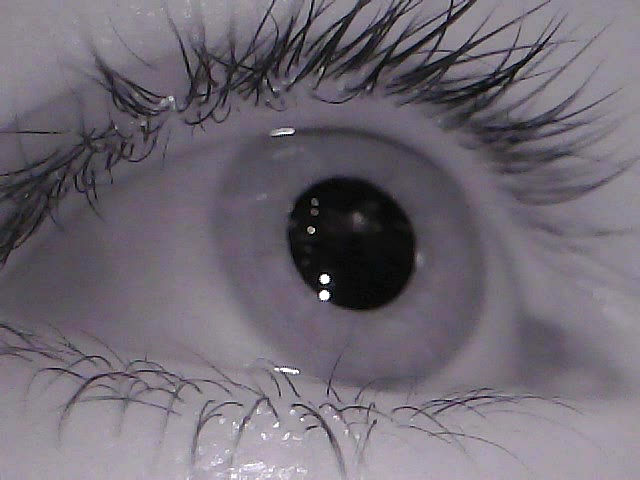
\includegraphics[width=.9\linewidth]{plots/eye_dataset/eye1.png}

      \label{fig:ds1}
    \end{subfigure}%
    \begin{subfigure}{.30\textwidth}
      \centering
      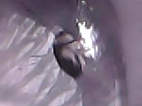
\includegraphics[width=.9\linewidth]{plots/eye_dataset/eye2.png}

      \label{fig:ds2}
    \end{subfigure}%
    \begin{subfigure}{.30\textwidth}
      \centering
      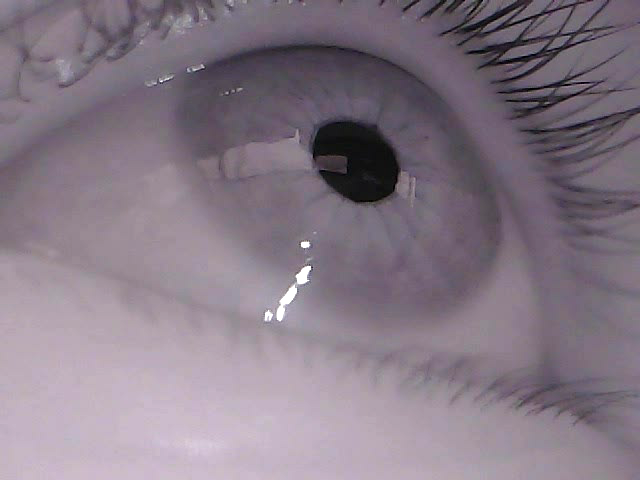
\includegraphics[width=.9\linewidth]{plots/eye_dataset/eye3.png}

      \label{fig:ds3}
    \end{subfigure}
    \caption{three example frames from the LPW data set.}
    \label{fig:example_frame}
    \end{figure}

    \subsection{Procedure}
    The participants were asked to look at a moving red ball as it moved around. The recording location was randomly picked and was in and around several buildings. Each location was chosen only once. 

    